\section{Aufbau und Durchführung}
\label{sec:Durchführung}
\subsection{Vorbereitende Justierungen}
Zu Beginn werden die gekoppelten Schwingkreise auf die gleiche Resonanzfrequenz
abgestimmt. Dazu wird eine Schaltung wie in Abbildung \ref{fig:abstimmung}
aufgebaut.
\begin{figure}
  \centering
  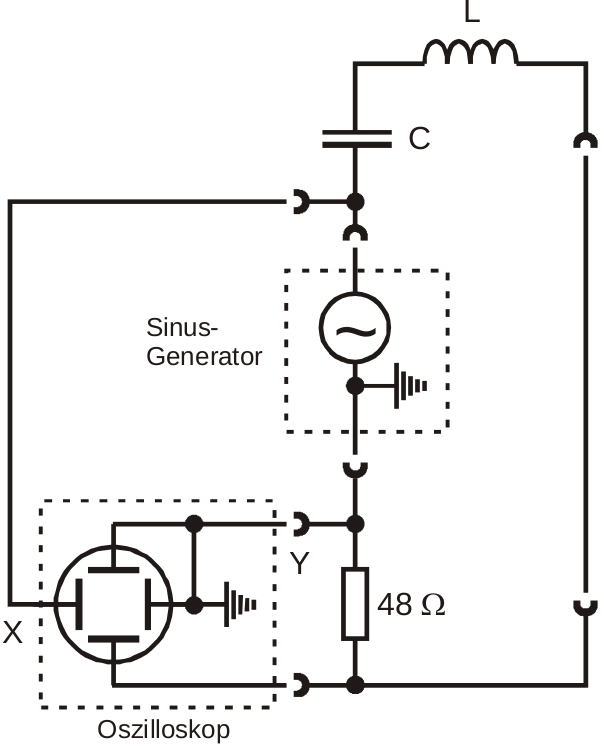
\includegraphics[width=0.5\textwidth]{abstimmung_neu.png}
  \caption{Schaltung zur Abstimmung der Resonanzfrequenz \cite{sample}.}
  \label{fig:abstimmung}
\end{figure}
Die Frequenz wir zunächst an dem Schwingkreis mit dem festen Kondensator eingestellt,
indem man die Frequenz so wählt, dass die Stromamplitude maximal ist. Genauer
eingestellt wir die Resonanzfrequenz, indem mit Hilfes eines Oszilloskops im
xy-Betrieb die Lissajous-Figuren so eingestellt werden, dass die Phasendifferenz
$\Delta \Phi = 0$ ist (die Lissajous-Figur ist dann ein Strich). Danach wird der
Kondensator des abstimmbaren Schwingkreises so eingestellt, dass die Resonanzfrequenz
möglichst ähnlich der im festen Schwingkreis eingestellten Resonanzfrequenz ist
(jedoch nicht exakt gleich).

\subsection{Verhältnis der Schwingungsfrequzenzen}
\label{sec:verhaeltnis}
Mit einem Rechtecksignal einer um etwa zwei Größenordnungen kleineren Frequenz
als der Resonanzfrequenz wird der in Abbildung \ref{fig:messung1} linke Schwingkreis
angeregt.
\begin{figure}
  \centering
  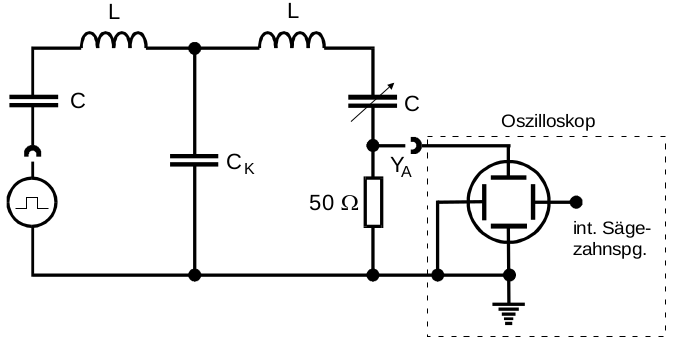
\includegraphics[width=0.9\textwidth]{messung1.png}
  \caption{Schaltung zur Untersuchung der Schwebung \cite{sample}.}
  \label{fig:messung1}
\end{figure}
Die Energie wird nun über den Koppelkondensator $C_\text{K}$ in den
rechten Schwingkreis (und wieder zurück) übertragen. Der zeitliche Verlauf des
Stromes im zweiten Schwingkreis wird mit einem Oszilloskop dargestellt. Dort
werden für jeden Kopplungskondensator die Schwingungsmaxima innerhalb einer
Schwingungsperiode abgezählt und das Verhältnis zwischen Schwingungs- und
Schwebungsfrequzen berechnet.

\subsection{Fundamentalfrequenzen in Abhänigkeit des Kopplungskondensators}
Die Schaltung aus Abschnitt \ref{sec:verhaeltnis} wird mit einem Sinussignal
angeregt. Es wird die Generatorspannung gegenüber der Spannung im Schwingkreis
mit einem Oszilloskop im xy-Betrieb beobachtet. Für jeden Kopplungskondensator
werden mit Hilfe der Lissajous-Figuren die Frequenzen $\nu^{+}$ (bei einer Phase
von $\Delta \Phi = 0$, hier ist die Lissajous-Figur eine Gerade) und $\nu^{-}$
(bei einer Phase von $\Delta \Phi = \pi$, hier ist die Lissajous-Figur ebenfalls
eine Gerade, jedoch an der y-Achse gespiegelt) gesucht und notiert.

\subsection{Verlauf der Ströme}
Mit dem Funktionsgenerator wird ein Sweep von $\SI{1}{\second}$ durchgeführt,
d.h. in einer Sekunde wird das Frequenzspektrum zwischen der eingestellten
Anfangs- und Endfrequenz kontinuierlich durchlaufen. Der Verlauf der Ströme kann
wieder mit einem Oszilloskop dargestellt werden. Mit der Hold-Funktion wird ein
Durchlauf auf dem Bildschirm angezeigt. Dort werden die Zeitdifferenzen zwischen
Start und erstem Maximum ($\Delta t_1$) und Start und zweitem Maximum ($\Delta t_2$)
wiederum für alle verschiedenen Kopplungskondensatoren gemessen.
